\subsection{General Architecture}
\label{sec:CG-Architecture}

As many \IOT solutions, \IOTDSL massively relies on event processing. In order to transform abstract event definitions into runnable code, we rely on a middleware on which the event processing will run and that will be responsible for the evaluation of the rules. Figure~\ref{fig:gen-archi} depicts the general architecture of the \IOTDSL framework.

\begin{figure}%
	\centering  
	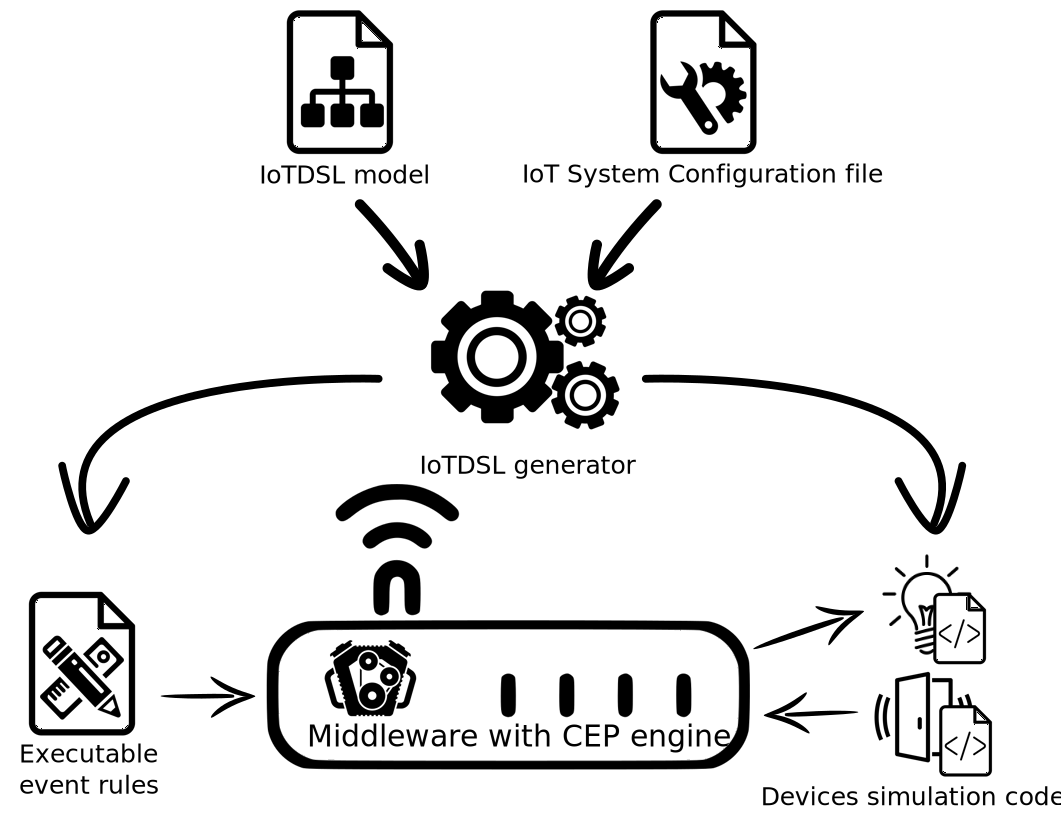
\includegraphics[width=.95\linewidth]{gen-archi.png}%
	\caption{General architecture of \IOTDSL framework}%
	\label{fig:gen-archi}%
\end{figure}

From \IOTDSL models, the generator will create a set of files that gathers, on the one side, all business rules as executable complex events and on the other side, a set of simulation code files used to emulate the device behaviours.